\chapter*{附錄一、MTi-G感測器精度測試}
\addcontentsline{toc}{chapter}{附錄一、MTi-G感測器精度測試}
MTi-G整合了許多不同的感測器,利用軟體運算的方式增進位置量測值的準確度。
因此MTi-G的精度測試將分為靜態測試與動態測試,測試其性能。

由於MTi-G所量測到的位置資訊為經緯度,但經緯度無法較直覺的比較準確度,
因此每一次實驗都是將所有的量測值取平均後得到一平均位置,利用此平均位置將所有的量測值換算為X方向與Y方向的距離並繪製圖表,
以公尺為單位比較每次實驗的結果。

\section*{靜態測試}
靜態測試是將MTi-G放置於室外一定點,記錄約30分鐘的位置資訊與Yaw角度資訊,並觀察其分佈。
由於是靜止不動的狀態,因此MTi-G此時並無法利用其它的感測資訊增進位置資訊的準確度。

靜態測試的結果如圖~\ref{f:app:stationary_test_1}與~\ref{f:app:stationary_test_2}所示,
左側為單位換算為公尺後位置資訊,右側則為時間(橫軸)與Yaw角(縱軸)的關係。
位置資訊之標準差及衛星個數如表~\ref{t:app:stationary_result}所示。
\begin{figure}[h!]
	\centering
	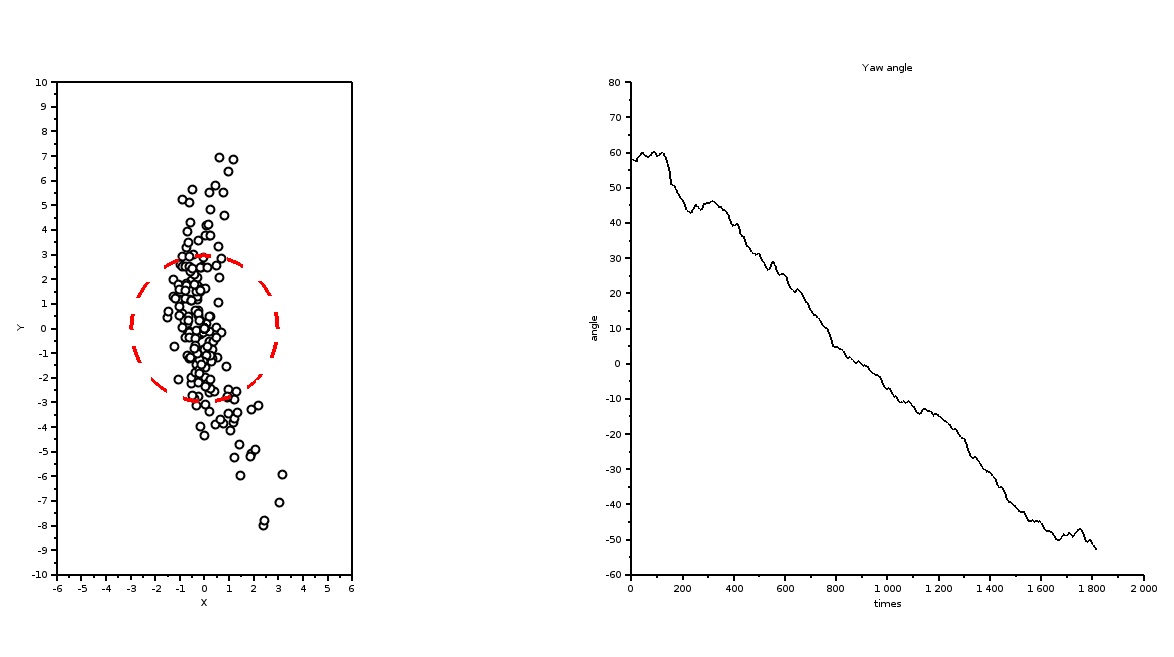
\includegraphics[width=\textwidth]{figures/appendix1/stationary_test_1}
	\caption{靜態測試實驗結果一}
	\label{f:app:stationary_test_1}
\end{figure}

\begin{figure}[h!]
	\centering
	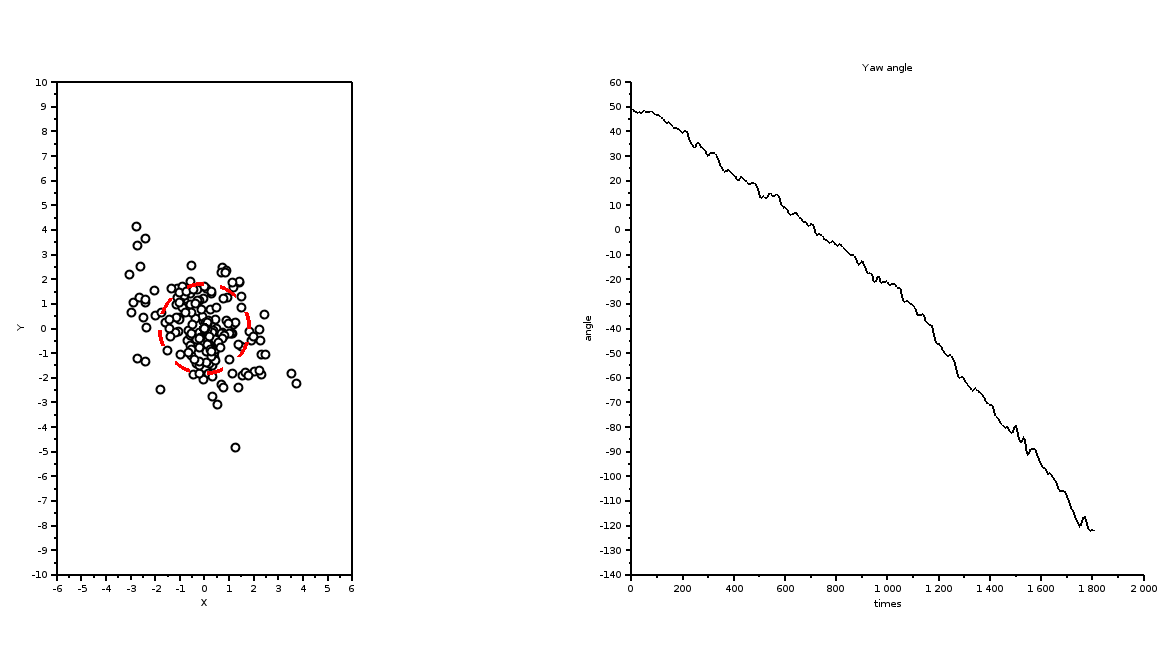
\includegraphics[width=\textwidth]{figures/appendix1/stationary_test_2}
	\caption{靜態測試實驗結果二}
	\label{f:app:stationary_test_2}
\end{figure}

\begin{table}[h!]
	\centering
	\caption{靜態測試結果比較}
	\label{t:app:stationary_result}
	\begin{tabular}{| l | c | c |}
		\hline
		 		& 位置資訊之標準差(m)	& 平均衛星數 \\ \hline
		第一次測試	& 2.967			& 8.14 \\ \hline
		第二次測試	& 1.819			& 7.92 \\
		\hline
	\end{tabular}
\end{table}

由靜態測試可看出兩個結果:第一,在沒有其它感測器補償的情況下,其位置精度並沒有顯著增加;
第二,若是沒有其它感測器的補償,Yaw角度會不斷偏移,無法收斂。

\section*{動態測試}
動態測試方法是將MTi-G裝置於Yun-Trooper II上,使用遙控的方式控制Yun-Trooper II以不同的路徑通過地面上的同一個位置,
並在通過該點的同時記錄當下量測到的位置資訊,重覆此動作約10次後計算其偏差,如圖~\ref{f:app:dynamic_env}所示。
\begin{figure}
	\centering
	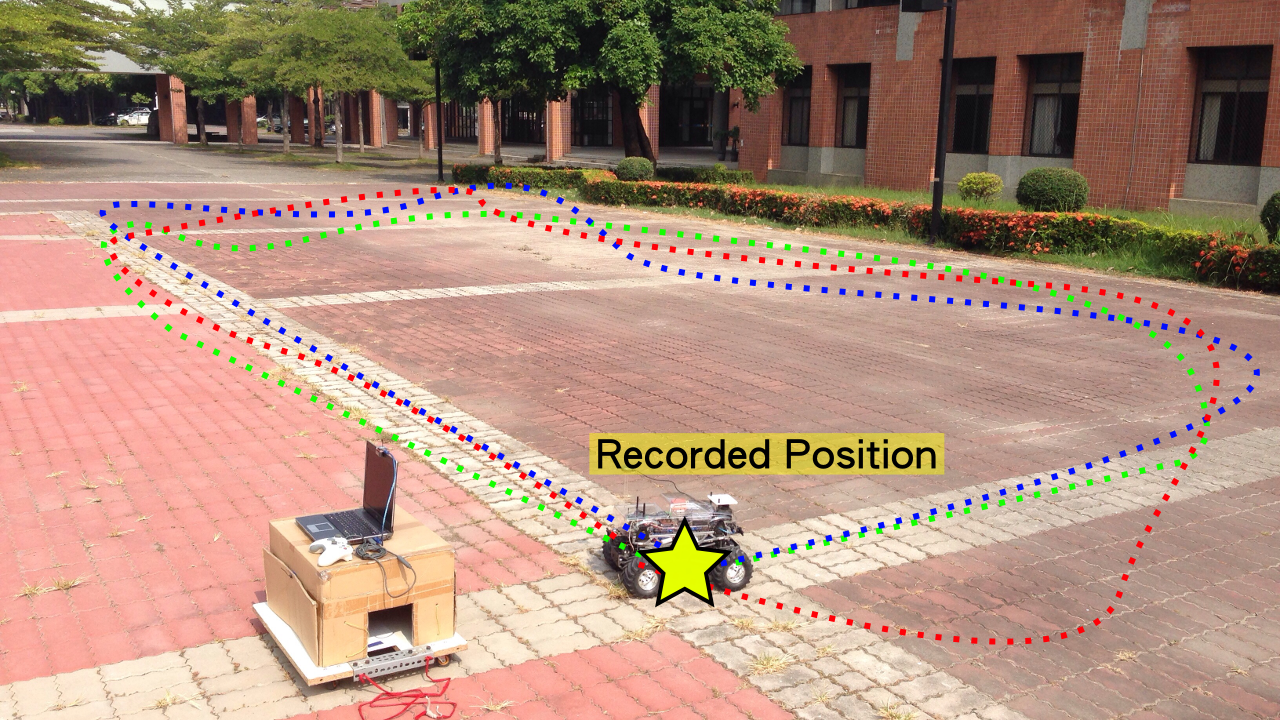
\includegraphics[width=\textwidth]{figures/MTiGTest/MTiG_env}
	\caption{動態測試示意圖}
	\label{f:app:dynamic_env}
\end{figure}

此方式讓MTi-G能夠取得除了GPS以外的感測器資訊,讓MTi-G能夠使用其它感測器資訊增進位置資訊的準確度。
另外,為了測試時間對MTi-G位置量測的影響,此實驗分別於每一天中的三個不同時段進行實驗,分別為10:30、15:30及20:30,
並於2014/04/22、2014/04/23與2014/04/24這三天進行此實驗。實驗結果如圖~\ref{f:app:dynamic_1}至圖~\ref{f:app:dynamic_9}所示,
而上述的同一位置點則使用$\times$標示於圖中,其標準差則使用紅色虛線圓圈表示。
所有實驗的位置資訊之標準差及衛星個數如表~\ref{t:app:dynamic_result}所示。

\begin{figure}[h!]
	\centering
	\begin{subfigure}[t]{0.32\textwidth}
		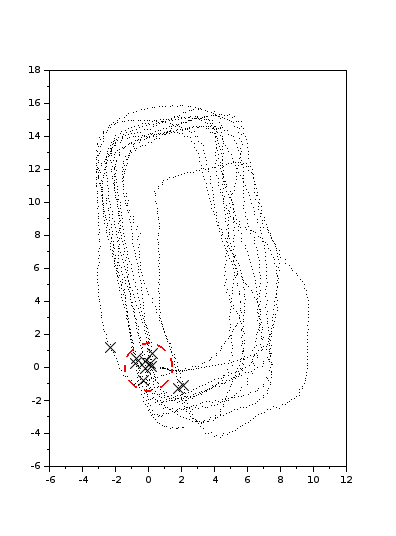
\includegraphics[width=\textwidth]{figures/appendix1/dynamic_1}
		\caption{10:30實驗結果}
		\label{f:app:dynamic_1}
	\end{subfigure}
	\begin{subfigure}[t]{0.32\textwidth}
		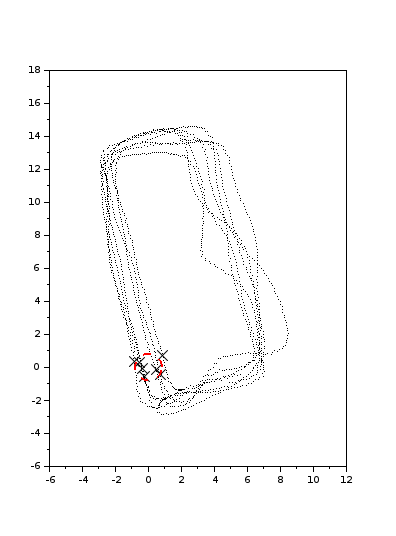
\includegraphics[width=\textwidth]{figures/appendix1/dynamic_2}
		\caption{15:30實驗結果}
		\label{f:app:dynamic_2}
	\end{subfigure}
	\begin{subfigure}[t]{0.32\textwidth}
		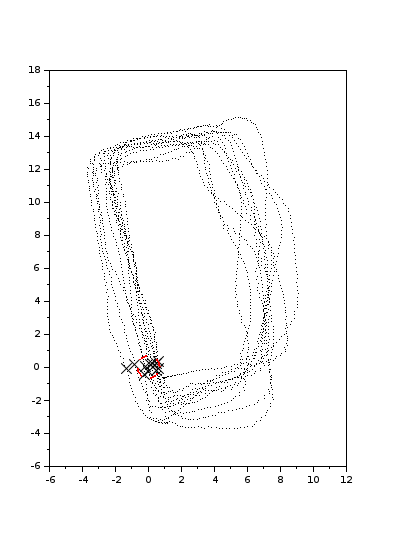
\includegraphics[width=\textwidth]{figures/appendix1/dynamic_3}
		\caption{20:30實驗結果}
		\label{f:app:dynamic_3}
	\end{subfigure}
	\caption{2014/04/22實驗結果}
\end{figure}
\begin{figure}[h!]
	\centering
	\begin{subfigure}[t]{0.32\textwidth}
		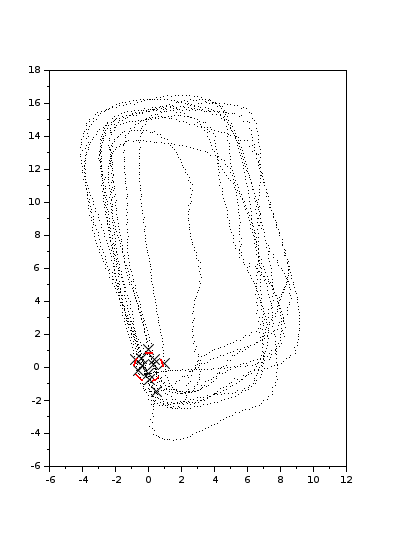
\includegraphics[width=\textwidth]{figures/appendix1/dynamic_4}
		\caption{10:30實驗結果}
		\label{f:app:dynamic_4}
	\end{subfigure}
	\begin{subfigure}[t]{0.32\textwidth}
		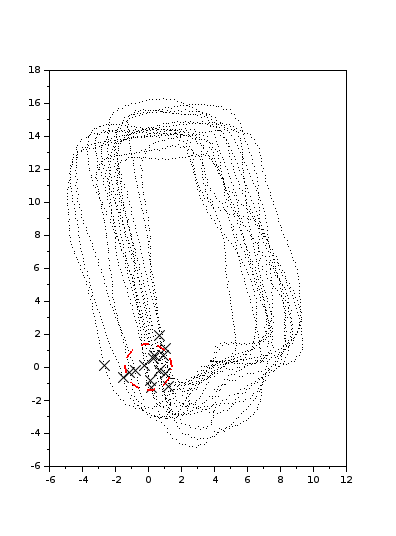
\includegraphics[width=\textwidth]{figures/appendix1/dynamic_5}
		\caption{15:30實驗結果}
		\label{f:app:dynamic_5}
	\end{subfigure}
	\begin{subfigure}[t]{0.32\textwidth}
		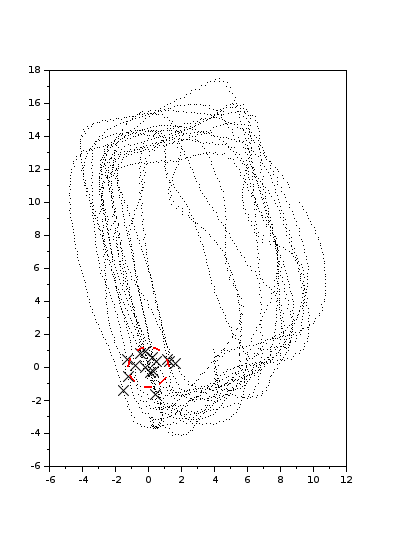
\includegraphics[width=\textwidth]{figures/appendix1/dynamic_6}
		\caption{20:30實驗結果}
		\label{f:app:dynamic_6}
	\end{subfigure}
	\caption{2014/04/23實驗結果}
\end{figure}
\begin{figure}[h!]
	\centering
	\begin{subfigure}[t]{0.32\textwidth}
		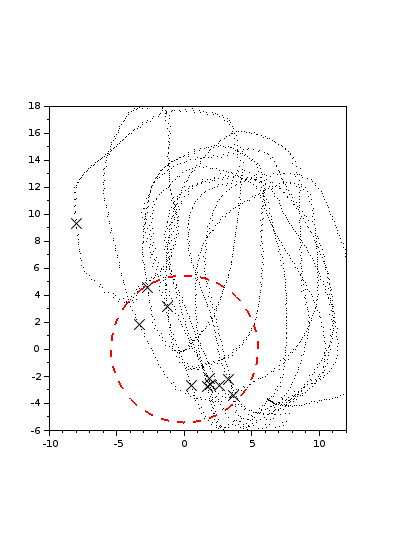
\includegraphics[width=\textwidth]{figures/appendix1/dynamic_7}
		\caption{10:30實驗結果}
		\label{f:app:dynamic_7}
	\end{subfigure}
	\begin{subfigure}[t]{0.32\textwidth}
		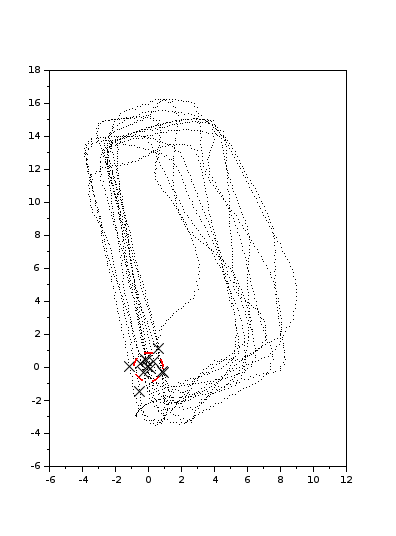
\includegraphics[width=\textwidth]{figures/appendix1/dynamic_8}
		\caption{15:30實驗結果}
		\label{f:app:dynamic_8}
	\end{subfigure}
	\begin{subfigure}[t]{0.32\textwidth}
		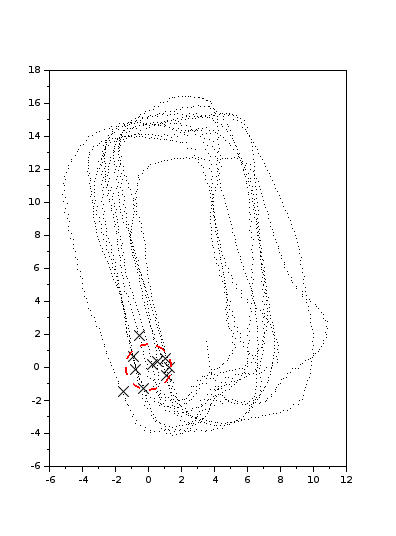
\includegraphics[width=\textwidth]{figures/appendix1/dynamic_9}
		\caption{20:30實驗結果}
		\label{f:app:dynamic_9}
	\end{subfigure}
	\caption{2014/04/24實驗結果}
\end{figure}

\begin{table}[h!]
	\centering
	\caption{動態測試結果比較}
	\label{t:app:dynamic_result}
	\begin{tabular}{| l | c | c |}
		\hline
		 	& 位置資訊之標準差(m)	& 平均衛星數 \\ \hline
		\multicolumn{3}{|c|}{2014/04/22} \\ \hline
		10:30	& 1.435			& 6.81 \\ \hline
		15:30	& 0.807			& 8.24 \\ \hline
		20:30	& 0.668			& 7.95 \\ \hline
		\hline
		\multicolumn{3}{|c|}{2014/04/23} \\ \hline
		10:30	& 0.871			& 5.92 \\ \hline
		15:30	& 1.400			& 5.76 \\ \hline
		20:30	& 1.217			& 7.90 \\ \hline
		\hline
		\multicolumn{3}{|c|}{2014/04/24} \\ \hline
		10:30	& 5.446			& 5.47 \\ \hline
		15:30	& 0.876			& 5.89 \\ \hline
		20:30	& 1.375			& 7.00 \\
		\hline
	\end{tabular}
\end{table}

從表~\ref{t:app:dynamic_result}可以看出,幾乎所有動態測試的位置準確度皆比靜態測試要好,
表示在其它感測器的輔助下的確可以增進位置資訊的準確度。然而,唯獨2014/04/24日10:30的實驗與其它結果差距相當大。

MTi-G利用軟體演算法,整合所有感測器的資訊後估測出當下的所有狀態(位置、姿態、速度等)。
因此,使用時必須等待其暖機完成(約15分鐘),並接收足夠的感測器資訊使估測結果收斂後才可使用,視情況這可能需要10至30分鐘不等的時間。
而2014/04/24日10:30的實驗便是在估測結果遲遲無法收斂的情況下所做的實驗結果,可以看到準確度相當低,甚至比靜態實驗還要差。
因此收斂與否對MTi-G的量測結果會造成相當大的影響。

為了測試時間對位置量測結果的影響,接下來於同一張圖,以顏色與圖案分別表示每一次實驗的結果,如圖~\ref{f:app:timediff}所示。
不同的圖案代表不同的實驗日期,而不同的顏色則代表了同一日期但不同時間點的實驗結果,而每個實驗皆有一虛線圓,其半徑即為該次實驗所得到的標準差。
\begin{figure}[h!]
	\centering
	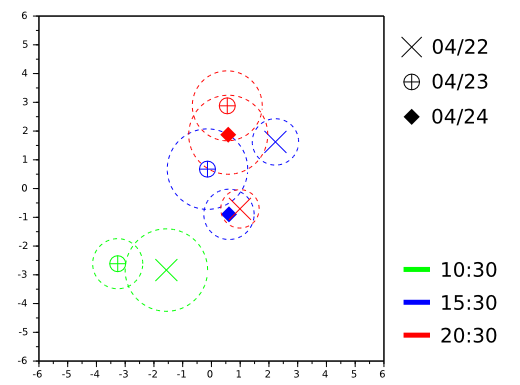
\includegraphics[width=0.8\textwidth]{figures/appendix1/timediff.png}
	\caption{時間對量測結果之影響}
	\label{f:app:timediff}
\end{figure}

從圖~\ref{f:app:timediff}可看到,時間的確會對MTi-G的位置量測結果造成影響,不同時間點的量測結果可能會有相當大的差異。
但因為MTi-G主要還是由GPS所獲得的位置資訊來估計位置,而GPS的精度會受到相當多的因素影響,因此MTi-G會有如此表現是可接受的。

另外,動態實驗的平均衛星個數與量測標準差之間的關係如圖~\ref{f:app:Sigma-N}所示,其中橫軸為平均衛星個數,縱軸為標準差。
因此若衛星數與量測準確度有關係存在,則衛星數越多量測標準差應該越小。然而從圖中可觀察到,衛星的個數與量測的準確度並沒有絕對的關係。
\begin{figure}[t!]
	\centering
	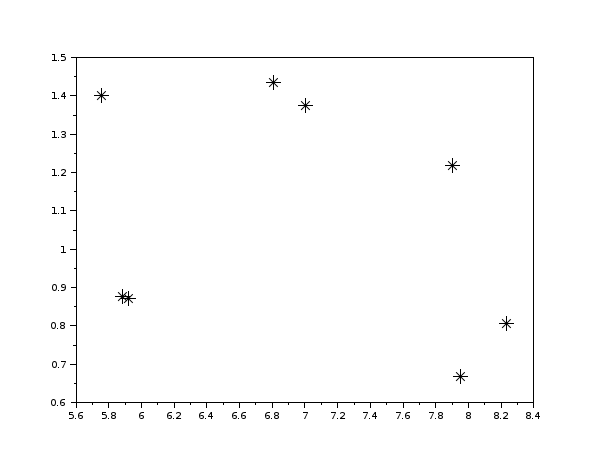
\includegraphics[width=0.8\textwidth]{figures/appendix1/Sigma-N}
	\caption{衛星數與量測標準差之關係圖}
	\label{f:app:Sigma-N}
\end{figure}

